\documentclass[12pt]{beamer}
\usepackage{../latex-sty/mypres}
\usepackage[utf8]{inputenc}
\usepackage[T2A]{fontenc}
\usepackage[english]{babel}

\expandafter\def\expandafter\insertshorttitle\expandafter{%
  \insertshorttitle\hfill%
  \insertframenumber\,/\,\inserttotalframenumber}
\title[Seminar 10]{Optimization methods. \\
 Seminar 10. Optimality conditions.}
\author{Alexandr Katrutsa}
\institute{Moscow Institute of Physics and Technology\\
Department of Control and Applied Mathematics} 
\date{\today}

\begin{document}
\begin{frame}
\maketitle
\end{frame}

\begin{frame}{Remainder}
\begin{itemize}
\item Conjugate function
\item Young-Fenchel inequality
\item Examples
\end{itemize}
\end{frame}

\begin{frame}{Motivation}

\begin{block}{Question \# 0}
When does solution of the optimization problem exist?
\end{block}

\begin{block}{Question \# 1}
How to check that a point is a solution of the optimization problem? 
\end{block}

\begin{block}{Question \# 2}
What conditions can give solution of the optimization problem?
\end{block}

\end{frame}

\begin{frame}{Existence of the solution}
\begin{block}{Weierstrass theorem}
Let $X \subset R^n$ be a compact set and $f: X \to \bbR$ be a continuous function on its domain.
Then the global minimizer of $f$ exists.
\end{block}

This theorem guarantees existence of the solution for most meaningful optimization problems
 
\end{frame}

\begin{frame}{Optimality conditions}
\begin{block}{Definition}
Optimality condition is a statement that gives necessary and/or sufficient condition for point to be local minimizer
\end{block}
Class of problems:
\begin{itemize}
\item General minimization problem
\item Unconstrained minimization problem 
\item Equality constrained minimization problems
\item Equality and inequality constrained minimization problem
\end{itemize}
\end{frame}

\begin{frame}{General minimization problem}

\begin{block}{Problem}
\[
f(x) \rightarrow \min\limits_{{\color{red}{x \in X}}}
\]
\end{block}

\begin{block}{Optimality criterion}
Assume $f(x)$ has domain $\mathrm{dom} \ f = X \subset \bbR^n$.
Then 
\begin{enumerate}
\item if $x^*$ is a local minimizer of $f(x)$, then $0 \in \partial_X f(x^*)$
\item if subdifferential $\partial_X f(x^*)$ exists in some point $x^* \in X$ and $0 \in \partial_X f(x^*)$, then $x^*$ is a local minimizer of $f(x)$.
\end{enumerate}
\end{block}
What drawbacks have this criterion?

\end{frame}

\begin{frame}{Examples}
\begin{itemize}
\item $\bx^{\T}\bx + \alpha \| \bx - 
\bc \|_2 \rightarrow \min\limits_{\bx \in \bbR^n}$, $\alpha > 0$
\item $\bx^{\T}\bx + \alpha \| \bc^{\T}\bx - 
b \|_2 \rightarrow \min\limits_{\bx \in \bbR^n}$, $\alpha > 0$
\item Constraint on feasible set
\begin{equation*}
\begin{split}
\vspace{-4mm}
&(x + 2)^2 + |y + 3| \rightarrow \min\limits_{(x, y) \in \bbR^2}\\
\text{s.t. }& 8 + 2x - y \leq 0
\end{split}
\end{equation*}
\end{itemize}
\end{frame}

\begin{frame}{Unconstrained minimization problem}
Problem: $f(x) \rightarrow \min\limits_{\color{red}{x \in \bbR^n}}$.

\begin{block}{Optimality criterion for convex functions}
Let $f: \bbR^n \to \bbR$ be a convex function.
Then $x^*$ is a solution of the unconstrained minimization problem iff $0 \in \partial f(x^*)$.
\end{block}

\begin{block}{Corollary}
If $f(x)$ is convex and differentiable, then $x^*$ is a solution of the problem iff $\nabla f(x^*) = 0$.
\end{block}

\begin{block}{Sufficient condition for non-convex functions}
Let $f: \bbR^n \to \bbR$ be twice differentiable and $x^*$ such that $\nabla f(x^*) = 0$. 
If  $\nabla^2 f(x^*) \succ 0$, then $x^*$ is a strict local minimizer.  
\end{block}

\end{frame}

\begin{frame}{Examples}
\begin{itemize}
\item $x_1e^{x_1} - (1 + e^{x_1})\cos x_2 \rightarrow \min$
\item Rosenbrock function: $(1 - x_1)^2 + \alpha \sum\limits_{i = 2}^n (x_i - x^2_{i-1})^2 \rightarrow \min$, $\alpha > 0$
\item $x^2_1 + x^2_2 - x_1x_2 + e^{x_1 + x_2} \rightarrow \min$
\end{itemize}
\end{frame}

\begin{frame}{{\small Equality constrained minimization problem}}

\begin{block}{Minimization problem}
\vspace{-5mm}
\begin{equation*}
\begin{split}
& f(x) \rightarrow \min\limits_{x \in \bbR^n} \\
\text{s.t. } & g_i(x) = 0, \; i = 1,\ldots, m 
\end{split}
\end{equation*}
\end{block}

\begin{block}{Lagrangian}
\vspace{-2mm}
\begin{equation*}
L(x, \blambda) = f(x) + \sum\limits_{i=1}^m\lambda_i g_i(x)
\end{equation*}
\end{block}

\begin{block}{Optimality condition (sufficient)}
Let $f(x)$ and $g_i(x)$ be twice differentiable functions in $x^*$ and continuously differentiable in some neighbourhood of $x^*$.
Assume that $\nabla_x L(x^*, \blambda) = 0$.
The if $\bh^{\T}\nabla^2 L(x^*, \blambda)\bh > 0$, where $\bh \in T(\bx^*|G)$~--- tangent cone, then $x^*$~--- point of the local minimum.
\end{block}

\end{frame}

\begin{frame}{Possible options}
\begin{figure}
\centering
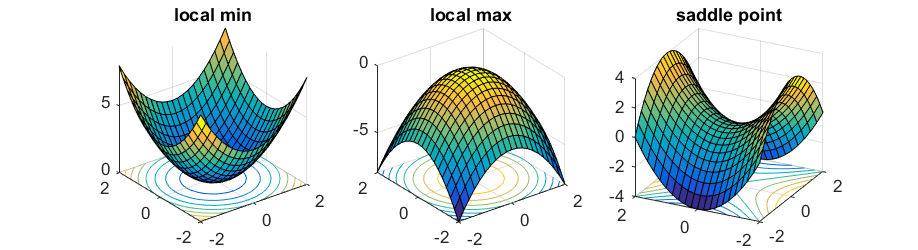
\includegraphics[scale=0.5]{minmaxsaddle.png}
\caption{Figure is from \url{http://www.offconvex.org/2016/03/22/saddlepoints/}}
\end{figure}
\end{frame}

\begin{frame}{Examples}
\begin{itemize}
\item $\sum\limits_{i=1}^n\alpha_i x^4_i \rightarrow \extr\limits_{\bx \in G}$, $G = \{\bx \in \bbR^n \; | \; \bc^{\T}\bx = 1 \}$, $\alpha_i > 0,\; c_i > 0$
\item $x_1 + 4x_2 + 9x_3 \rightarrow \extr\limits_{\bx \in G}, \; G = \left \{ \frac{1}{x_1} + \frac{1}{x_2} + \frac{1}{x_3} = 1 \right\}$
\end{itemize}
\end{frame}

\begin{frame}{{\small Equality and inequality constrained minimization problem}}

\begin{block}{Minimization problem}
\vspace{-5mm}
\begin{equation*}
\begin{split}
& \min\limits_{x \in \bbR^n} f(x)\\
\text{s.t. } & g_i(x) = 0, \; i = 1,\ldots,m\\
& h_j(x) \leq 0, \; j = 1,\ldots, p
\end{split}
\end{equation*}
\end{block}

\begin{block}{Lagrangian}
\begin{equation*}
L(x, \blambda, \bmu) = f(x) + \sum\limits_{i=1}^m\lambda_i g_i(x) + \sum\limits_{j=1}^p \mu_j h_j(x)
\end{equation*}
\end{block}
\end{frame}

\begin{frame}{Optimality conditions}
\begin{block}{Necessary condition (Karush - Kuhn - Tucker)}

Пусть $x^*$ решение задачи математического программирования, и функции $f, h_j, g_i$ дифференцирумы. 
Тогда найдутся такие $\bmu^*$ и $\blambda^*$, что выполнены следующие условия:
\begin{itemize}
\item $g_i(x^*) = 0$, $i = 1,\ldots,m$
\item $h_j(x^*) \leq 0$, $j = 1,\ldots,p$
\item $ \mu^*_j \geq 0$, $j = 1,\ldots,p$
\item $\mu^*_jh_j(x^*) = 0$, $j = 1,\ldots,p$
\item $\nabla_x L(x^*, \blambda^*, \bmu^*) = 0$
\end{itemize}
\end{block}
If the minimization problem is convex, then the necessary optimality condition is also sufficient.
\end{frame}

\begin{frame}{Optimality conditions (cont'd)}
\small
If the problem in non-convex, then
\begin{block}{First order sufficient condition}
\small
If a stationary point $(x^*, \blambda^*, \bmu^*)$ gives number of active constraints $|J|$ such that $n = m + |J|$ and $\mu_j > 0, \; j \in J$, then this point is local minimizer.
\end{block}

\begin{block}{Second order sufficient condition}
\small
If the number of active constraints is less than the dimension of the, then $x^*$ is a local minimizer if the following conditions hold
\vspace{-3mm}
\[
\bz^{\T}\nabla_{xx}^2 L(x^*)\bz > 0
\vspace{-3mm}
\] 
for 
\vspace{-4mm}
\begin{itemize}
\item $\bz \neq 0$ и $\nabla g^{\T}_i(x^*)\bz = 0$
\vspace{-3mm}
\item $j \in J$ and $\mu_j > 0$, $\nabla h^{\T}_j(x^*) \bz = 0$
\vspace{-3mm}
\item $j \in J$ and $\mu_j = 0$, $\nabla h^{\T}_j(x^*) \bz \leq 0$
\end{itemize}
\end{block}

\end{frame}

\begin{frame}{Examples}
\begin{itemize}
\small
\item Example 1
\vspace{-5mm}
\begin{equation*}
\begin{split}
& \extr (x_1 - 3)(x_2 - 2)\\
\text{s.t. } & x_1 + 2x_2 = 4\\
& x^2_1 + x^2_2 \leq 5\\
& x_1 \geq 0, \; x_2 \geq 0 
\end{split}
\end{equation*} 
\vspace{-5mm}
\item Example 2
\vspace{-5mm}
\begin{equation*}
\begin{split}
& \extr \sum\limits_{i=1}^n \frac{c_i}{x_i}\\
\text{s.t. } & \sum\limits_{i=1}^n a_ix_i \leq b\\
& x_i > 0, \; b > 0, \; c_i > 0, \; a_i > 0
\end{split}
\end{equation*}
\vspace{-4mm}
\item Example 3
\vspace{-3mm}
\begin{equation*}
\begin{split}
& \extr (x_1x_3 - 2x_2)\\
\text{s.t. } & 2x_1 - x_2 - 3x_3 \leq 10\\
& 3x_1 + 2x_2 + x_3 = 6\\
& x_2 \geq 0
\end{split}
\end{equation*}
\end{itemize}
\end{frame}

\begin{frame}{Recap}
\begin{itemize}
\item Existence of the solution of the minimization problem
\item Optimality conditions for
\begin{itemize}
\item general minimization problem
\item unconstrained minimization problem
\item equality constrained minimization problem 
\item equality and inequality constrained minimization problem
\end{itemize}
\end{itemize}
\end{frame}
\end{document}
